\section{IEEE 802.15.7 - PHY \rmnum{3}}
\label{sec:ieeestd}
\graphicspath{{_MIMOColor/figures_csk/}}
LED based luminaires are energy efficient and are thus being widely adopted in indoor spaces to provide illumination. In order to dynamically control the rendered illumination spectrum, luminaires contain multiple elements of at least three colors of LEDs. Different SPDs can be rendered by mixing different ratios of radiant flux emitted from the multiple LEDs comprising a luminaire. Each resulting SPD realizes a different color mix to the human eye.

Any SPD within the visible range of electromagnetic spectrum can produce a stimulus when incident on the sensors of the human eye (rod and cones) and has a color associated with it. This color can also be represented by its intensity, hue and saturation. While intensity is a measure of the total power comprising the SPD, hue and saturation are subjective parameters analogous to mean and spread of the wavelengths comprising the SPD and are quantified by a chromaticity coordinate. The \textit{commission internationale de l'eclairage} (CIE) has specified the CIE 1931 XYZ color space (CIE-CS) that provides a mathematical model to represent the chromaticity of radiation in the visible range as a point in a 2-dimensional plane. Let a luminaire be comprised of three types of LEDs, namely LED$_{n}$; $n\in$ \text{\{i, j, k\}}. The chromaticity of each LED can be represented by a coordinate ($x_{n}$, $y_{n}$) on the CIE-CS. When different intensities of radiant flux emitted by three types of LEDs are combined, the chromaticity coordinate of the resultant SPD will lie inside the triangle formed by coordinates of the LEDs themselves.

\renewcommand{\arraystretch}{1.1}
\begin{table}[t]
\centering
\begin{tabular}{|c|c|c|c|c|}
\hline
\multirow{2}{*}{\textbf{CB$_{u}$}} & \textbf{Band} & \textbf{Center} & \multirow{2}{*}{\textbf{x}} & \multirow{2}{*}{\textbf{y}}\\
 & \textbf{(nm)} & \textbf{(nm)} & & \\
\hline
CB$_{0}$ & 380 - 478 & 429 & 0.169 & 0.007\\
\hline
CB$_{1}$ & 478 - 540 & 509 & 0.011 & 0.733\\
\hline
CB$_{2}$ & 540 - 588 & 564 & 0.402 & 0.597\\
\hline
CB$_{3}$ & 588 - 633 & 611 & 0.669 & 0.331\\
\hline
CB$_{4}$ & 633 - 679 & 656 & 0.729 & 0.271\\
\hline
CB$_{5}$ & 679 - 726 & 703 & 0.734 & 0.265\\
\hline
CB$_{6}$ & 726 - 780 & 753 & 0.734 & 0.265\\
\hline
\multicolumn{5}{c}{ }
\end{tabular}
\caption{Color bands as outlined in IEEE 802.15.7}
\label{tCB}
\end{table}
\renewcommand{\arraystretch}{1.0}

\begin{figure}[!t]
\centering
		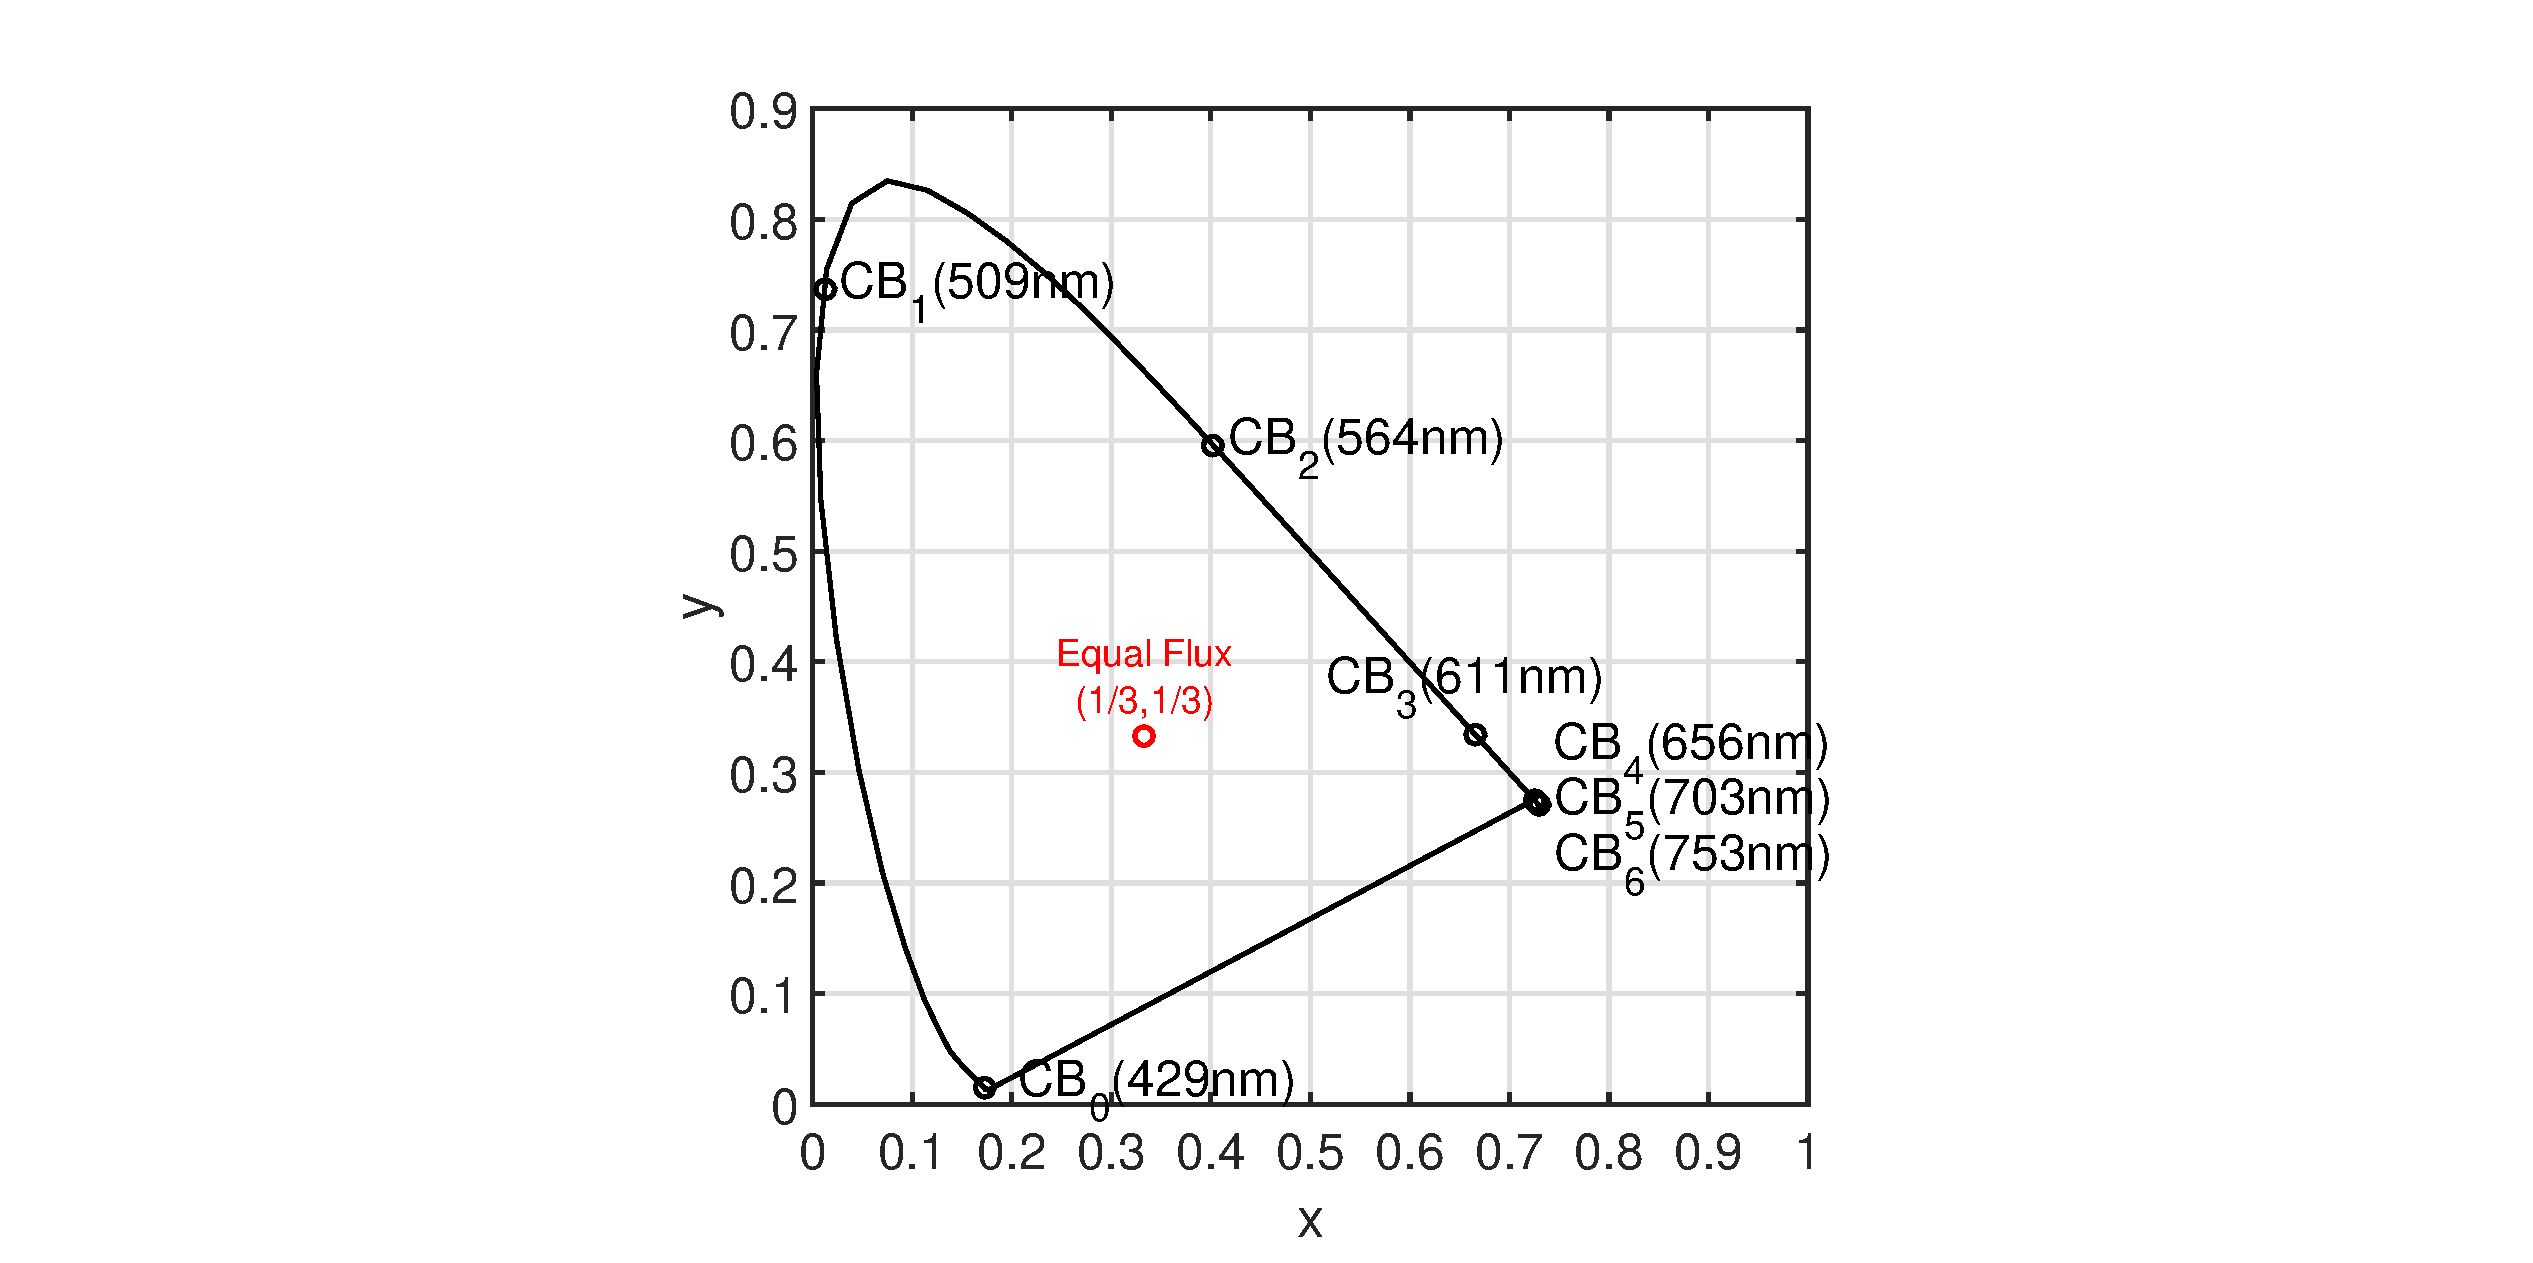
\includegraphics[trim={4.3in 0in 4.3in 0.5in}, clip=true, width=3.0in]{CBCcenters.eps}
	\caption{Color band centers on CIE-CS}
	\label{figCBCcenters}
\end{figure}


The IEEE standard for short-range OWC using visible light specifies CSK as the modulation technique of choice under the PHY \rmnum{3} specifications \cite{IEEE802.15.7}. For the rest of this chapter, the noun `standard' shall imply the IEEE 802.15.7 standard, specifically chapter 12 on PHY \rmnum{3} specifications. The standard outlines linear system configurations with $M$-ary CSK to achieve up to 96 Mb/s data rate. Reference \cite{raj12a} provides an overview of modulation and dimming techniques specified within the standard while reference \cite{sin13a} studies select color bands for CSK.

CSK is a modulation technique in which information is transmitted through changes in chromaticity coordinates. This can be achieved by varying the intensities of LED$_{n}$ over time. To select sources for CSK implementation, the standard specifies 7 different color bands - CB$_{u}$; $0\leq u < 7$ by splicing the visible spectrum range into 7 contiguous segments as shown in Table \ref{tCB}. The center wavelength of each segment as represented on CIE-CS is illustrated in \figurename{ }\ref{figCBCcenters}. Note that even though center wavelengths of CB$_{4}$, CB$_{5}$ and CB$_{6}$ are 47 nm -- 50 nm apart, the distance between their chromaticity coordinates is very small. The CIE-CS is designed such that the SPD resulting from identical flux emitted by the three primary sources maps to coordinate (1/3, 1/3) which is shown in \figurename{ }\ref{figCBCcenters}. We can define a color sector on the CIE-CS as the region enclosed by a color band on the perimeter and coordinate (1/3, 1/3). Though not explicitly mentioned in the standard, it is assumed that SPD of each LED$_{n}$ must belong to a different color sector. To study the performance of CSK independent of specific LED characteristics, it is generally assumed that the chromaticity coordinate of an LED belonging to a color sector corresponds to the center wavelength of a color band CB$_{u}$ at the perimeter of the sector as illustrated in \figurename{ }\ref{figCBCcenters}.

\renewcommand{\arraystretch}{1.1}
\begin{table}[t]
\centering
\begin{tabular}{|c|c|c|c|}
\hline
Color band combination & \multicolumn{3}{c|}{Color band '$u$' for CBC$_{v}$} \\
\cline{2-4}
\textbf{CBC$_{v}$} & \textbf{Band i} & \textbf{Band j} & \textbf{Band k} \\
\hline
CBC$_{1}$ & 6 & 2 & 0 \\
\hline
CBC$_{2}$ & 6 & 1 & 0 \\
\hline
CBC$_{3}$ & 5 & 2 & 0 \\
\hline
CBC$_{4}$ & 5 & 1 & 0 \\
\hline
CBC$_{5}$ & 4 & 2 & 0 \\
\hline
CBC$_{6}$ & 4 & 1 & 0 \\
\hline
CBC$_{7}$ & 3 & 2 & 0 \\
\hline
CBC$_{8}$ & 3 & 1 & 0 \\
\hline
CBC$_{9}$ & 2 & 1 & 0 \\
\hline
\end{tabular}
\caption{Color bands combinations as outlined in IEEE 802.15.7}
\label{tCBC}
\end{table}
\renewcommand{\arraystretch}{1.0}

\afterpage{%
\clearpage
\begin{landscape}% Landscape page
\renewcommand{\arraystretch}{1.1}
\begin{table}
\centering
\begin{tabular}{|c|c|c|c|}
\hline
\textbf{m} & \textbf{$M$ = 4} & \textbf{$M$ = 8} & \textbf{$M$ = 16} \\
\hline
0 & C$^{v}_{\text{j}}$ & (2C$_{4}$+C$_{5}$)/3 & C$^{v}_{\text{j}}$\\
1 & (C$^{v}_{\text{i}}$+C$^{v}_{\text{j}}$+C$^{v}_{\text{k}}$)/3 & (2C$_{a}$+C$_{b}$)/3; C$_{a}$=(C$_{b}$+C$_{3}$+C$_{5}$)/3; C$_{b}$=(C$_{4}$+C$_{5}$)/2 & (C$_{0}$+C$_{3}$+C$_{5}$)/3 \\
2 & C$^{v}_{\text{k}}$ & (2C$_{a}$+C$_{b}$)/3; C$_{a}$=(C$_{b}$+C$_{3}$+C$_{7}$)/3; C$_{b}$=(C$_{4}$+C$_{7}$)/2 & (C$_{3}$+C$_{6}$+C$_{10}$)/3 \\
3 & C$^{v}_{\text{i}}$ & (C$_{5}$+C$_{7}$)/2 & (2C$_{0}$+C$_{9}$)/3 \\
\cline{2-2}
4 & & C$^{v}_{\text{j}}$ & (C$_{0}$+2C$_{8}$)/3 \\
5 & & C$^{v}_{\text{k}}$ & (2C$_{0}$+C$_{8}$)/3 \\
6 & & (2C$_{4}$+C$_{7}$)/3 & (C$_{0}$+C$_{8}$+C$_{9}$)/3 \\
7 & & C$^{v}_{\text{i}}$ & (C$_{4}$+C$_{5}$+C$_{6}$)/3 \\
\cline{3-3}
8 & & & C$^{v}_{\text{i}}$ \\
9 & & & C$^{v}_{\text{k}}$ \\
10 & & & (C$_{0}$+2C$_{9}$)/3 \\
11 & & & (C$_{9}$+C$_{10}$+C$_{15}$)/3 \\
12 & & & (2C$_{8}$+C$_{9}$)/3 \\
13 & & & (C$_{4}$+C$_{8}$+C$_{12}$)/3 \\
14 & & & (C$_{6}$+C$_{12}$+C$_{15}$)/3 \\
15 & & & (C$_{8}$+2C$_{9}$)/3 \\
\hline
\end{tabular}
\caption[Design rules to compute constellation points for $M$-ary CSK]{Design rules to compute constellation points for $M$-ary CSK. Each row computes C$_{m}$, the chromaticity coordinate for m$^{th}$ codeword for any given CBC$_{v}$. C$^{v}_{n}$ is the chromaticity coordinate of color band $n\in$ \{i, j, k\} belonging to CBC$_{v}$.}
\label{tMCSK}
\end{table}
%Each row computes C$_{m}$, the chromaticity coordinate for m$^{th}$ codeword for any given CBC$_{v}$. C$^{v}_{n}$ is the chromaticity coordinate of color band $n\in$ \{i, j, k\} belonging to CBC$_{v}$.
\renewcommand{\arraystretch}{1.0}
\end{landscape}
\clearpage% Flush page
}

To implement CSK using 3 types of LEDs, the standard defines different sets of 3 color bands and calls each set a color band combination (CBC). The 3 different types of LEDs forming a CBC are ordered in a descending manner based on the center wavelength of the color band they belong to and each such band is called `band i', `band j' and `band k' respectively. 9 such CBC$_{v}$; $1\leq v\leq 9$ are defined in the standard and are outlined in Table \ref{tCBC}. The generalized notation CB$^{v}_{n}$ is used to indicate color band of type $n\in$ \text{\{i, j, k\}} belonging to CBC$_{v}$. Thus in Table \ref{tCBC}, the cell representing row for CBC$_{v}$ and column for band $n$ provides index $u$ for the color band represented by notation CB$^{v}_{n}$. Using this notation CB$^{1}_{\text{i}}$ $\equiv$ CB$_{6}$ while CB$^{2}_{\text{j}}$ $\equiv$ CB$_{1}$ and so on.

\afterpage{%
%\clearpage
%\begin{landscape}% Landscape page
\begin{figure}[!t]
	\centering
		\begin{subfigure}{\textwidth}
		\centering
			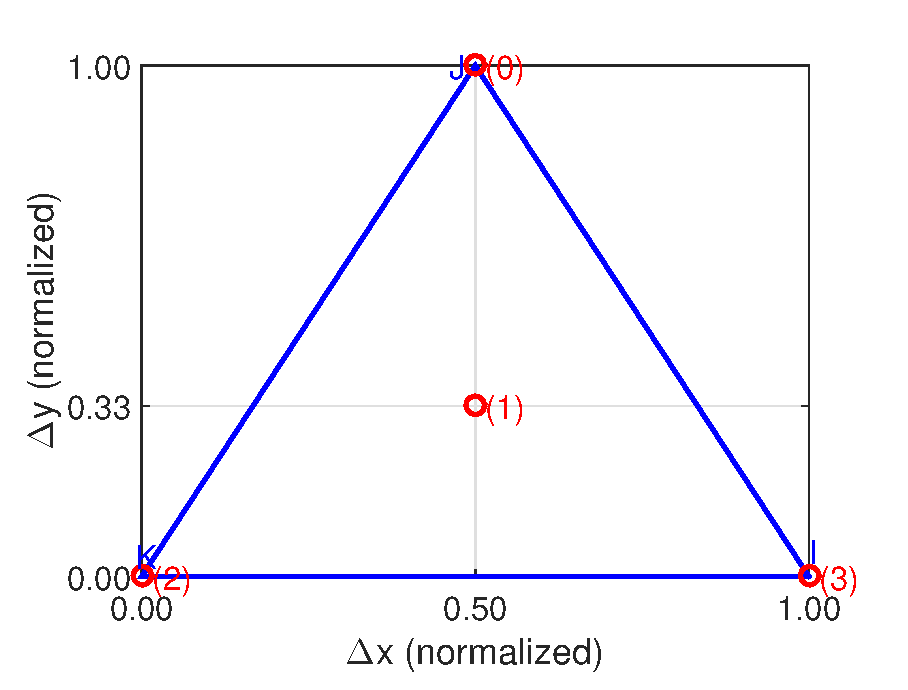
\includegraphics[trim={0.05in 0.0in 0.25in 0.2in}, clip=true, width=0.45\textwidth]{CBCrules4.eps}
			\caption{4-CSK}
			\label{fig4Const}
		\end{subfigure}
		\vfill
		\begin{subfigure}{\textwidth}
		\centering
			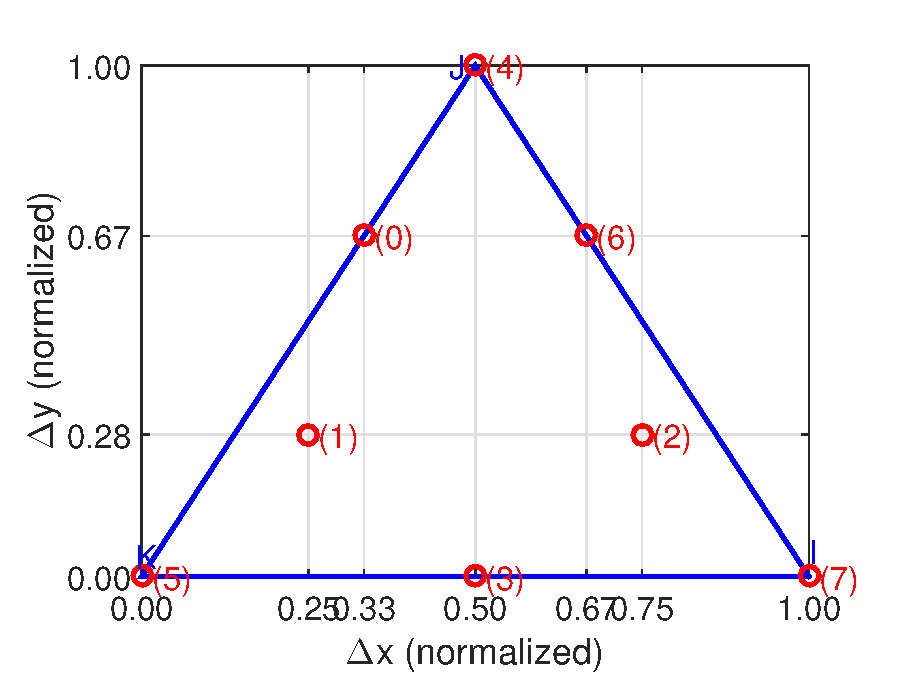
\includegraphics[trim={0.05in 0.0in 0.25in 0.2in}, clip=true, width=0.45\textwidth]{CBCrules8.eps}
			\caption{8-CSK}
			\label{fig8Const}
		\end{subfigure}
		\vfill
		\begin{subfigure}{\textwidth}
		\centering
			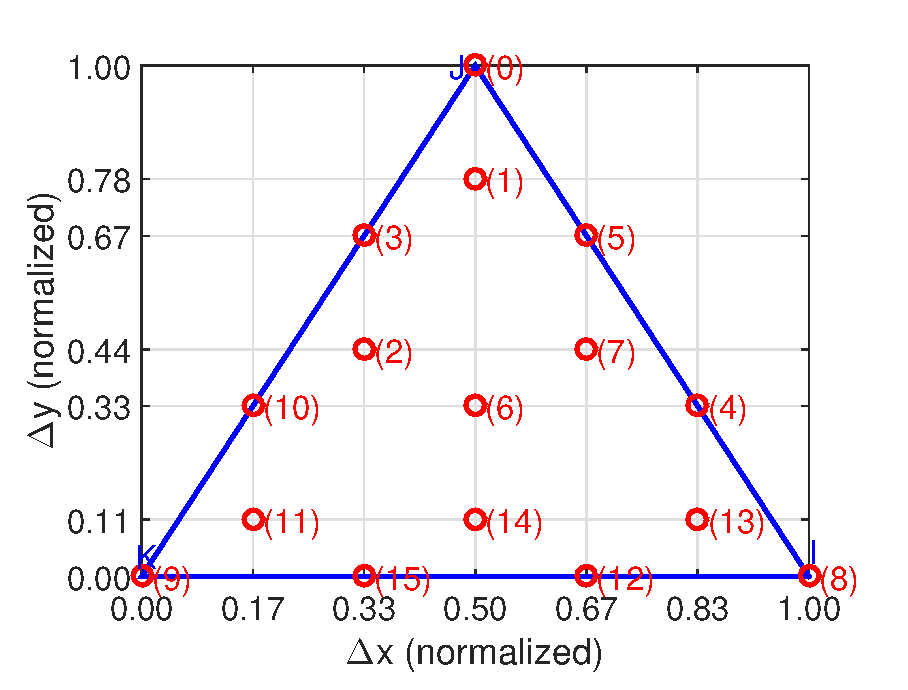
\includegraphics[trim={0.05in 0.0in 0.25in 0.2in}, clip=true, width=0.45\textwidth]{CBCrules16.eps}
			\caption{16-CSK}
			\label{fig16Const}
		\end{subfigure}
	\caption{$M$-ary CSK (normalized) constellation design rules}
	\label{figConst}
\end{figure}
%\end{landscape}
\clearpage% Flush page
}

For an $M$-ary CSK using CBC$_{v}$, the design rules to compute the $M$ different constellation points are provided in the standard and their values are outlined in \cite{cskxy}. Let C$^{v}_{n}$ $\equiv$ (x$^{v}_{n}$, y$^{v}_{n}$) be chromaticity coordinate corresponding to CB$^{v}_{n}$. Let C$_{m}$ $\equiv$ ($x_{m}$, $y_{m}$); $0\leq m <$ $M$ be chromaticity coordinate corresponding to m$^{th}$ codeword. Then Table 3 outlines the design rules for computing the constellation points. C$^{v}_{n}$ can be looked up from Table \ref{tCBC} and Table \ref{tCB}. Using these values, remaining C$_{m}$ can then be computed using rules from Table \ref{tMCSK}. Normalized constellation design rules for $M$-ary CSK are illustrated in \figurename{ }\ref{figConst}. Points I, J and K represent normalized coordinates for the $n$ color bands comprising a CBC. 

%\afterpage{%
%\clearpage
%\begin{landscape}% Landscape page
%
%\end{landscape}
%\clearpage% Flush page
%}